\documentclass{article}
\usepackage[utf8]{inputenc}
\usepackage[catalan]{babel}
\usepackage{amssymb}        % símbols de l'AMS
\usepackage{amsmath}        % macros de l'AMS
\usepackage[pdftex]{graphicx}  % poder incloure gráfics
\usepackage[pdftex]{color}     % poder fer servir color al text
\usepackage{multicol}
\usepackage{amsthm}
\usepackage{listings}
\usepackage{hyperref}
\usepackage{geometry}
\usepackage{tikz}
\usepackage{pgfplots}
\usepackage{subcaption}
\usepackage[catalan]{babel}
\usepackage{mathtools}
\usepackage{geometry}
\usepackage{amsmath}
\usepackage{amssymb}
\usepackage{fancyhdr}
\usepackage{multirow}
%\usepackage[table,xcdraw]{xcolor}
\usepackage{float}
\usepackage{verbatim}
\usepackage{pgfplots}
\pgfplotsset{compat=newest}
\usepgfplotslibrary{fillbetween}
\usetikzlibrary{patterns}
\usepackage{vmargin} 				%margenes



\title{Pràctica 2: Classificació}
\author{Guillermo Vivancos Alonso 1606206\\
	Javier Esmoris Cerezuela 1498396\\
	Oriol Marión Escudé 1566740}
\begin{document}
	\date{}
	\setpapersize{A4}
	\setmargins{2.5cm}       % margen izquierdo
	{1.5cm}                        % margen superior
	{16.5cm}                      % anchura del texto
	{23.42cm}                    % altura del texto
	{10pt}                           % altura de los encabezados
	{1cm}                           % espacio entre el texto y los encabezados
	{0pt}                             % altura del pie de página
	{2cm}                           % espacio entre el texto y el pie de página
	
	\pagestyle{fancy}
	\fancyhf{}
	\lhead{\textbf{Aprenentatge Computacional 102787} \newline Pràctica 2: Classificació\\}
	\rhead{\hfill \textbf{
			Guillermo Vivancos Alonso 1606206\\
			Javier Esmoris Cerezuela 1498396\\
			Oriol Marión Escudé 1566740}}
	\rfoot{\thepage}
	\maketitle
	\noindent
	\section*{Introducció}
	En aquesta pràctica analitzarem una base de dades sobre la potabilitat de l'aigua i les diferents concentracions d'algunes substàncies. Veurem quines distribucions tenen els atributs, la relació entre ells i intentarem determinar si donada una mostra, aquesta és potable o no.
	
	\section*{Apartat B}
	\textbf{Exploratory Data Analysis}\\
	\\
	Els atributs que tenim a la base de dades són els següents:
	\begin{enumerate}
		\addtocounter{enumi}{-1}
		\item pH [float]: pH de l'aigua.
		\item Hardness [float]:concentració de calci i magnesi.
		\item Solids [float]: edat del jugador mesurada en anys i dies.
		\item Chloramines [float]: concentració de cloramines. 
		\item Sulfate [float]: concentració de sulfats.
		\item Conductivity [float]: conductivitat de l'aigua.
		\item Organic\_carbon [float]: concentració de compostos orgànics.
		\item Trihalomethanes [float]: concentració de trihalometans.
		\item Turbidity [float]: Terbolesa de l'aigua.
		\item Potability [integer]: 0 si no és potable, 1 si és potable.
	\end{enumerate}
	Tenim 10 atributs a la base de dades, tots de tipus float menys l'últim que és binari, per tant l'atribut categòric només pot prendre dos valors.\\
	\\
	Pel que fa a les correlacions amb l'atribut categòric, totes són poc significatives com es pot veure en la figura~\ref{fig:correlacions}.\\
	\begin{figure}[!h]
		\centering
		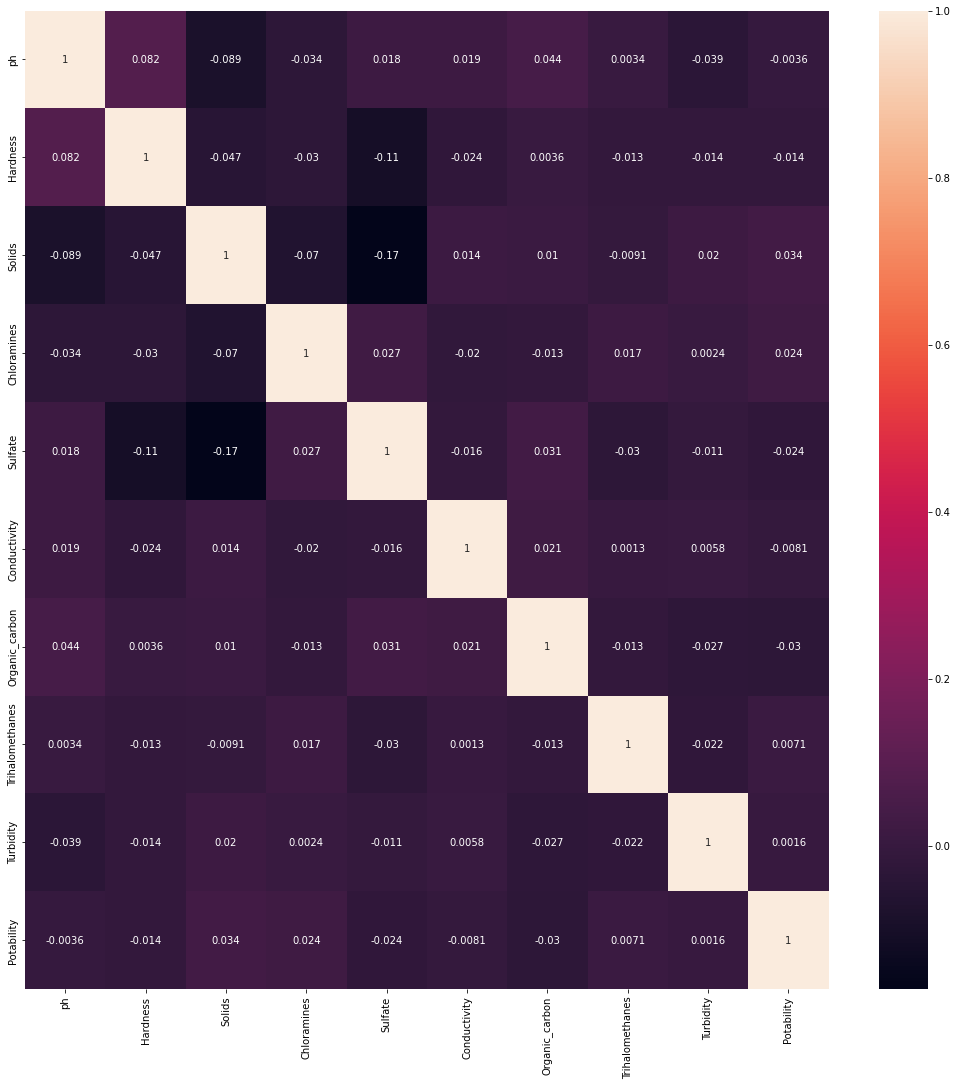
\includegraphics[width=0.4\linewidth]{../images/correlacions}
		\caption{Correlació entre els atributs}
		\label{fig:correlacions}
	\end{figure}\\
	A continuació veurem la distribució de la potabilitat~\ref{fig:distribuciopotabilitat} i les distribucions dels altres atributs segons la potabilitat~\ref{fig:distribucions}.\\
	\\
	\begin{figure}[!h]
		\centering
		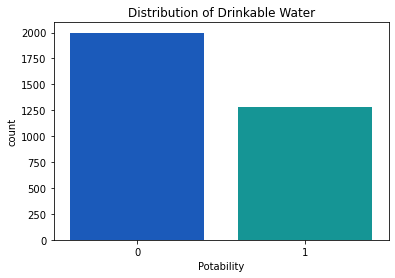
\includegraphics[width=0.4\linewidth]{../images/distribucio_potabilitat}
		\caption{Distribucio de la potabilitat}
		\label{fig:distribuciopotabilitat}
	\end{figure}
	\begin{figure}[!h]
		\centering
		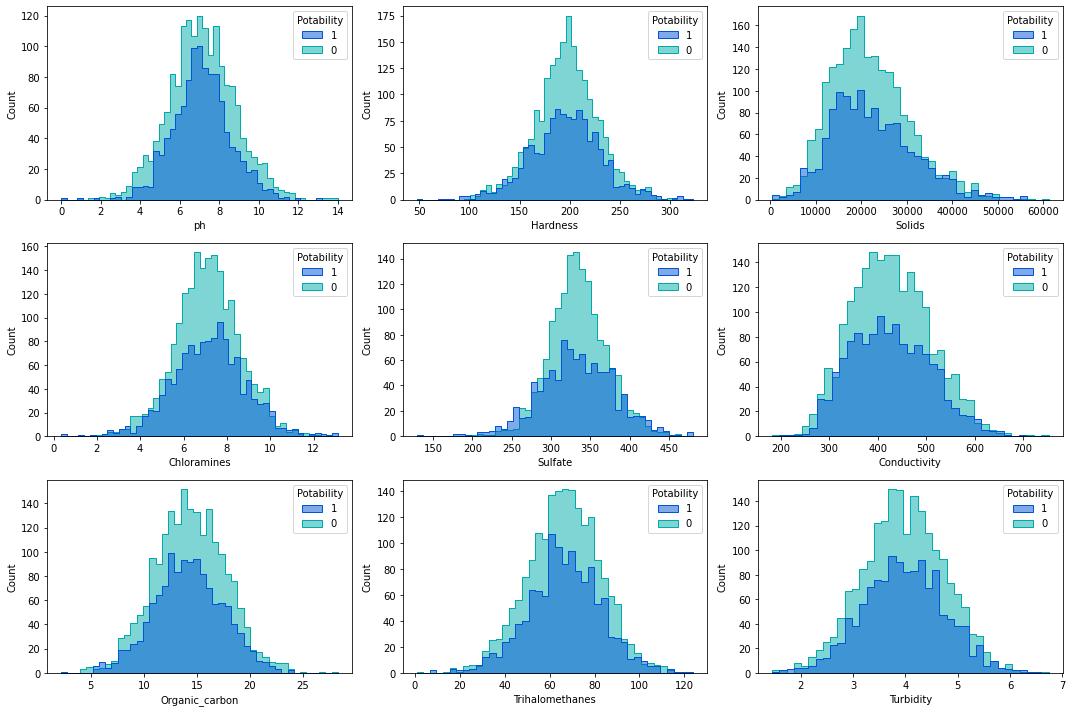
\includegraphics[width=0.7\linewidth]{../images/distribucions}
		\caption{Distribucions dels atributs segons la potabilitat}
		\label{fig:distribucions}
	\end{figure}\\
	A simple vista podem veure en la figura~\ref{fig:distribucions} que els atributs tenen una distribució gaussiana o pràcticament gaussiana. Les etiquetes de potabilitat estan balancejades (proporció 3:2).
	\clearpage
	\noindent
	\textbf{Preprocessing}\\
	\\
	En primer lloc mirem quines variables tenen NaNs, que són pH, Sulfate i Trihalomethanes. Els valors mitjans dels atributs, tant quan l'aigua és potable com no, són molt semblants, per tant, substituim els NaNs per la mitja dels atributs.\\
	\\
	La variable categòrica pren només dos valors, per tant tècniques com Ordinal Encoder o OneHotEncoder no tenen gaire sentit en aquest context.\\
	\\
	Hi ha rangs de variables molt aixos en comparació amb uns altres. L'atribut solids té el rang més alt de l'ordre de $6\cdot10^6$
	No tenim files repetides a la base de dades.\\
	\\
	
	
	
	
	
	\section*{Apartat A}

	
	
\end{document}